\section{Day 4: Graphing Example; Operations on Functions, Definition of Continuity by Open Sets (Sep. 11, 2024)}
We graphed $w = x^2 + y^2 - z^2$ in class today. Since I don't really know how to LaTeX these kinds of graphs, I'll just drop these pictures in;
\begin{figure}[h]
    \centering
    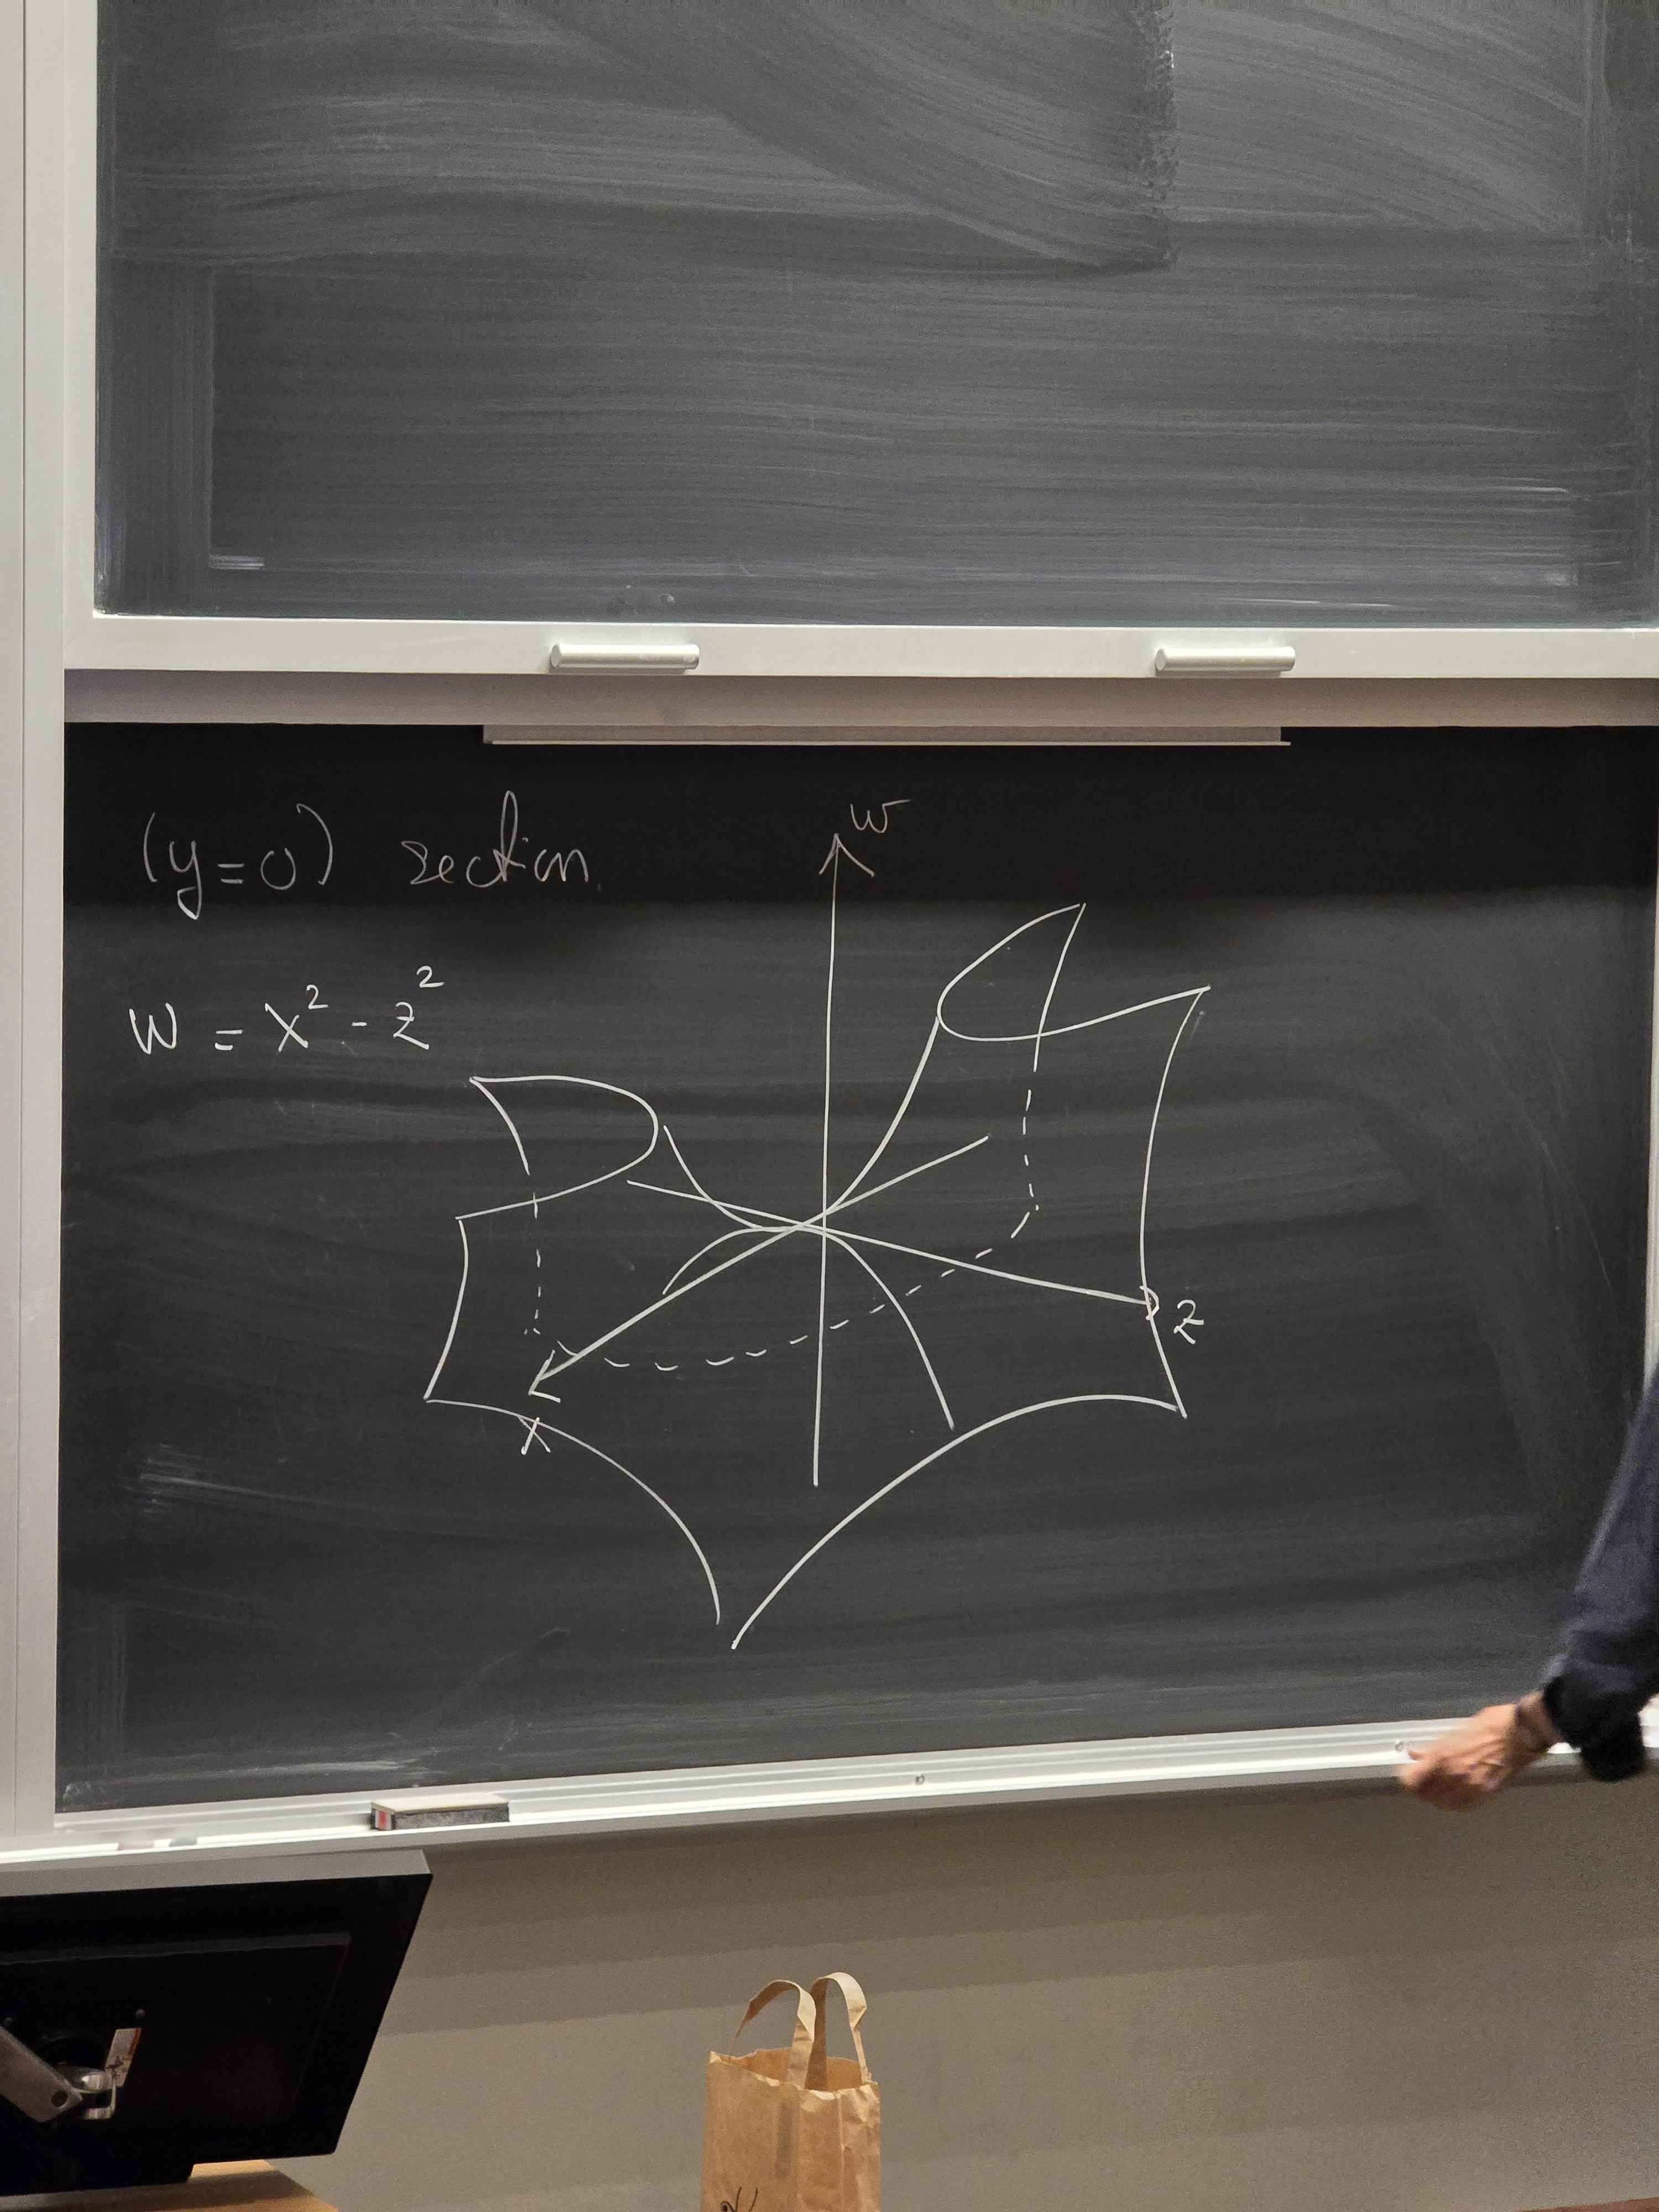
\includegraphics[scale=0.06]{MAT257 Notes/Diagrams/Day 4 Graph 1.jpg}
    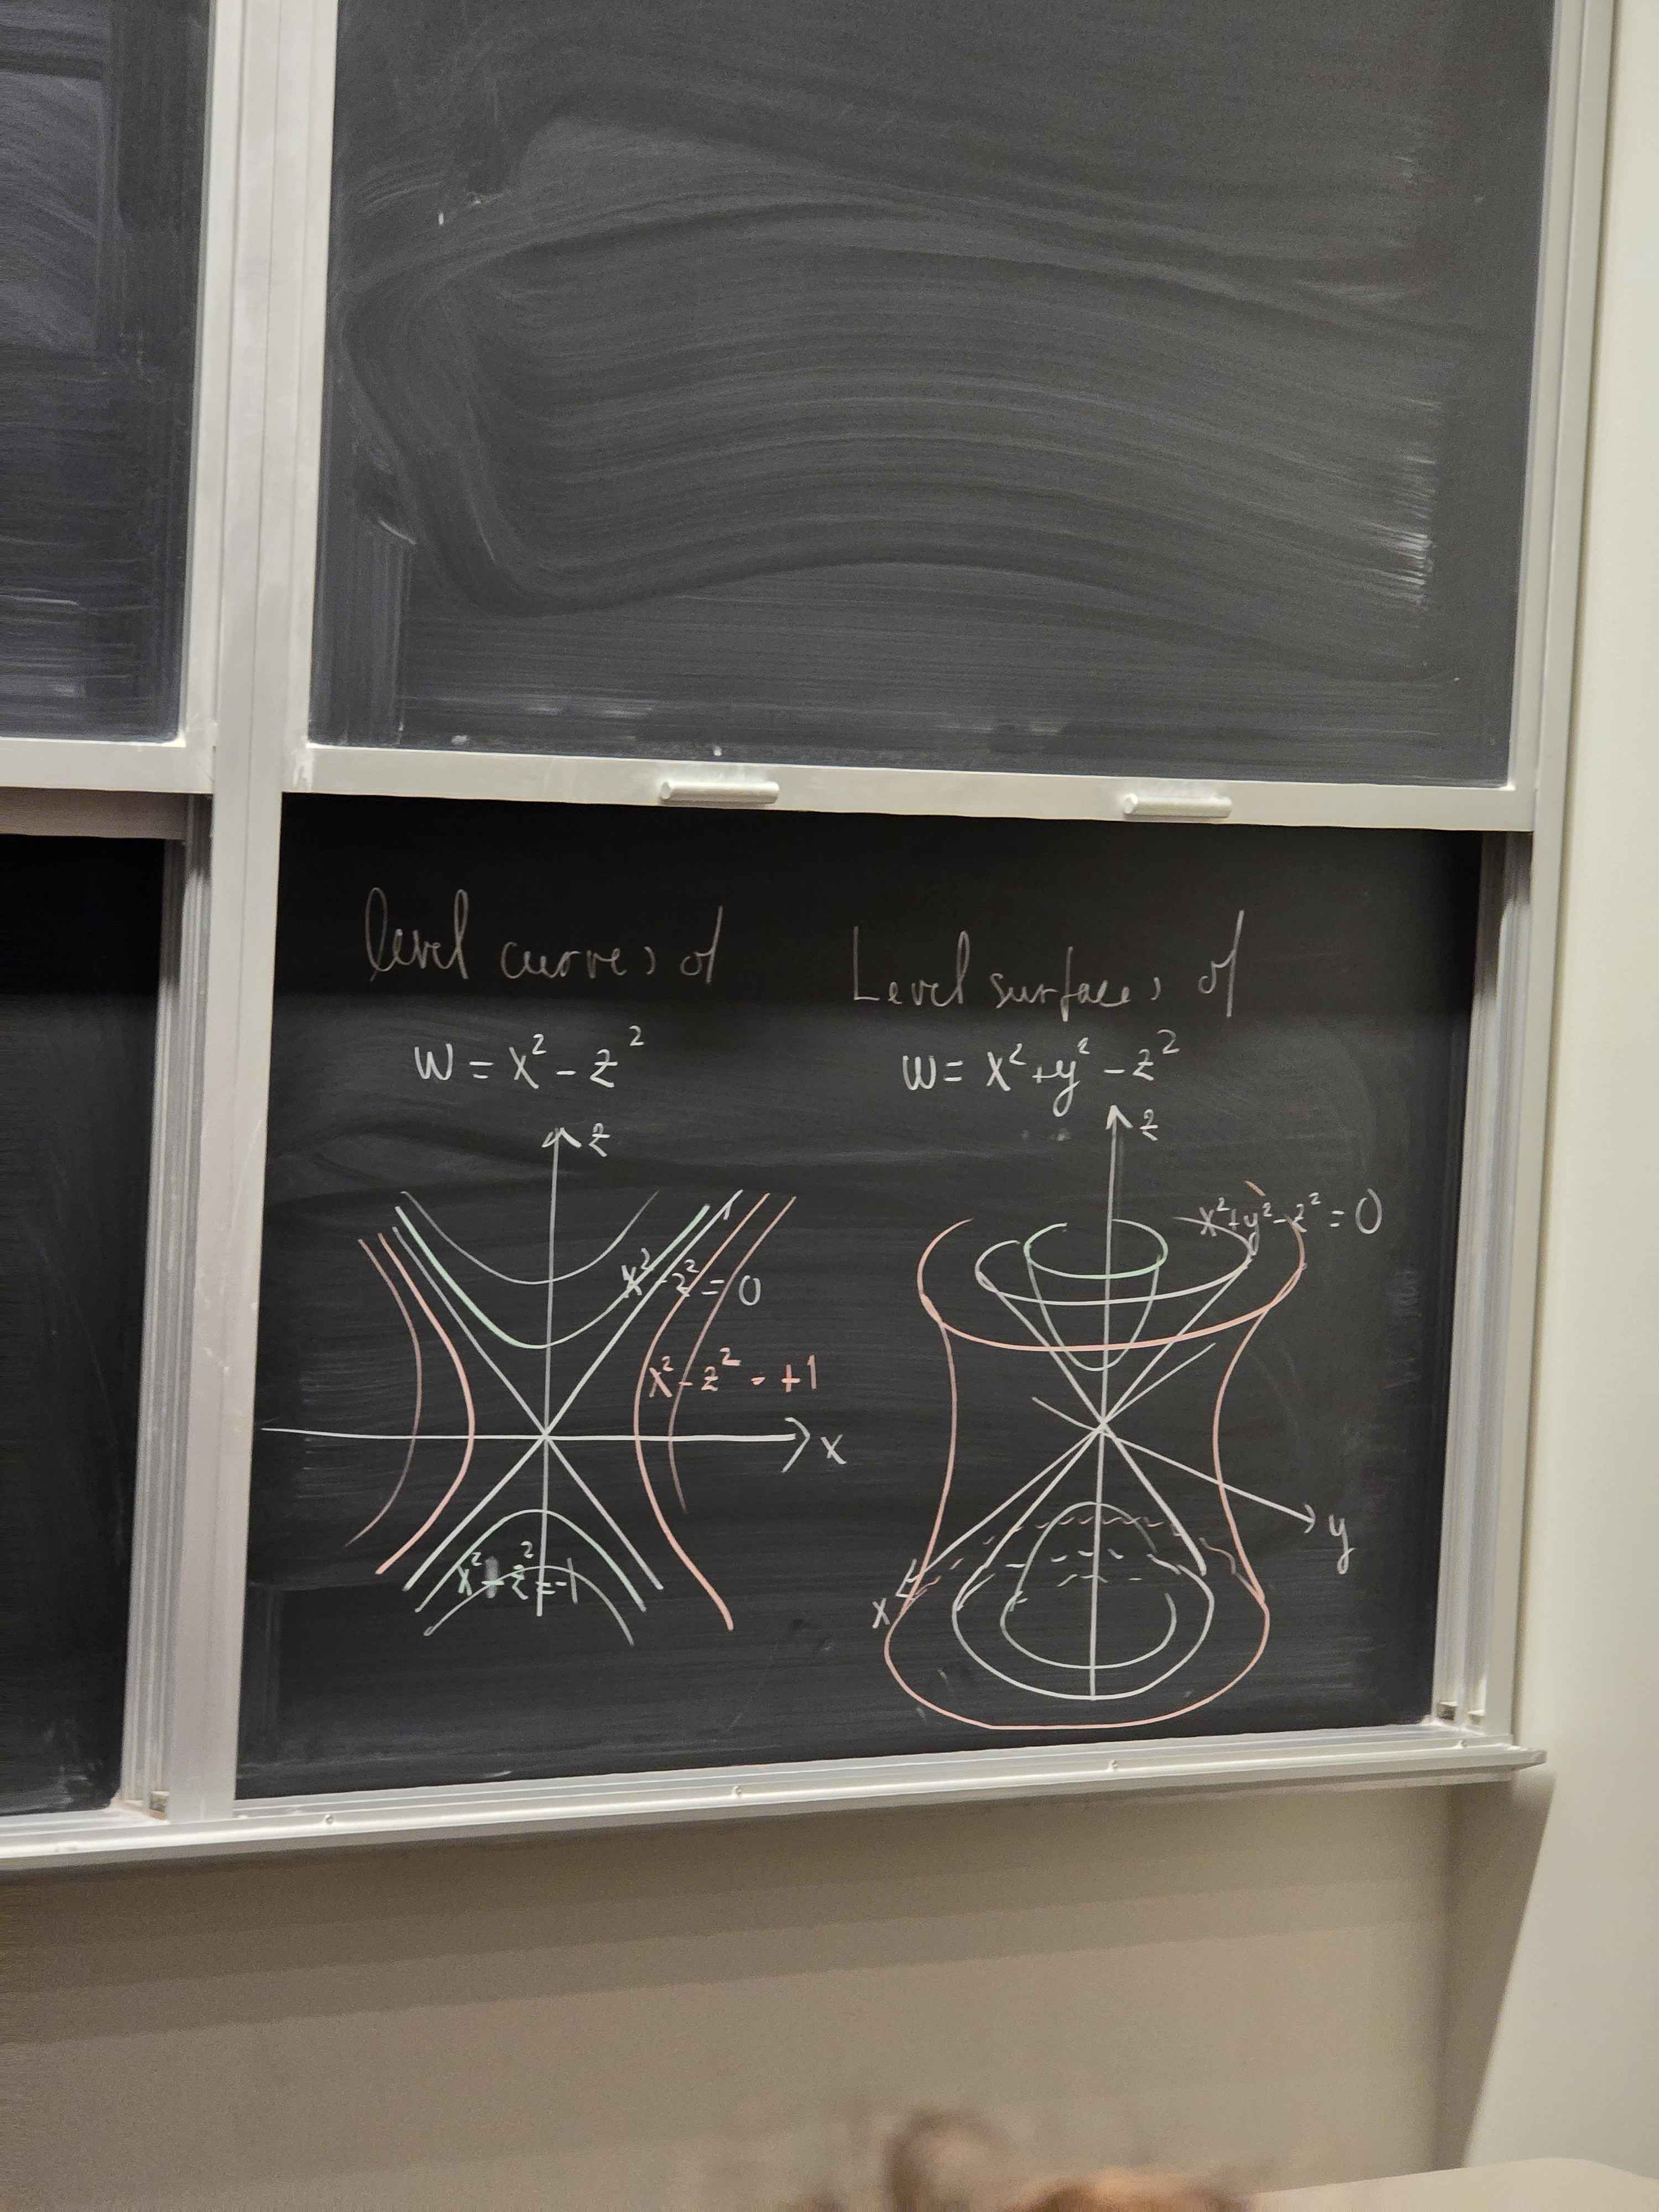
\includegraphics[scale=0.06]{MAT257 Notes/Diagrams/Day 4 Graph 2.jpg}
\end{figure}
\medskip\newline
\noindent The main idea was to start by considering $z = 0$ and observing that $w = x^2 + y^2$ is really a parabola ($w = x^2$, $w = y^2$) rotated about the $w$-axis; setting $x$ or $y$ to $0$, we get the left picture. If we examine the level sets of $w = x^2 - z^2$, we may combine the two to obtain the level surfaces of $w = x^2 + y^2 - z^2$ (as per the rightmost diagram on the blackboard).
\bigskip\hrule\bigskip
\noindent Let $A \subset \RR^n$, and consider a function $f : A \to \RR^m$ (i.e., a function $f : \RR^n \to \RR^m$ with domain restricted onto $A$). If we want to create another function $g : B \to \RR^p$ to be composed with $A$, we implicitly ask that $f(A) \subset B$; with this, we may write
\[ (g \circ f)(x) = g(f(x)) \]
where $\dom (g \circ f) = f^{-1}(B)$. Now, let us consider the inner product $\left< \, , \right> : \RR^m \times \RR^m \to \RR$. Let $f, g$ be functions from $\RR^n$ to $\RR^m$. Then we may construct
\begin{align*}
    (f, g)(x) &: \RR^n \to \RR^m \times \RR^m, \\
    f \cdot g &= \left< \, , \right> \circ (f \cdot g), 
\end{align*}
which we may indeed check sends $\RR^m \times \RR^m \to \RR$ as expected of the definition of dot product.
\medskip\newline
\noindent Returning to earlier, let us consider $f : (A \subset \RR^n) \to \RR^m$, and let us consider $f(x)$ written in its components, $f(x) = (f_1(x), \dots, f_m(x))$. If we wish to be specific, observe that we may write each $f_i$ as the following composition,
\[ f_i = \pi_i \circ f \text{ where } \pi_i : \RR^m \to \RR, \]
where $\pi_i$ is the mapping $(x_1, \dots, x_m) \mapsto x_i$.

\newpage
\noindent On the topic of limits, recall from MAT157 that $\lim_{x \to a} f(x) = b$ means that for every $\eps > 0$, there exists $\delta > 0$ such that if $x$ is in a $\delta$-ball of $a$, then $f(x)$ is in an $\eps$-ball of $b$. We may extend this idea to define continuity; we say $f$ is continuous at $a$ if
\[ \lim_{x \to a} f(x) = f(a), \]
and that $f$ is a continuous function if it is continuous for all $a \in A$. If we want to define continuity in its topological notion, though, we have that $f : \RR^n \to \RR^m$ is continuous if and only if $f^{-1}(U)$ is open in $\RR^n$ for all $U \subset \RR^m$.
\begin{simplethm}[Spivak 1.8]
    We say $f : (A \subset \RR^n) \to \RR^m$ is continuous if and only if, for all $U \subset \RR^m$, $f^{-1}(U) = A \cap V$ for some open set $V \subset \RR^n$.\footnote{do note that this proof is different from lecture, since i either mis-transcribed or bierstone made a mistake concerning balls for all $a \in A$ sending to $b$. }
\end{simplethm}
\begin{itemize}
    \item[$(\Rightarrow)$] Consider any open set $U \subset \RR^m$. If $a \in f^{-1}(U)$, we have $b := f(a) \in U$. Since $U$ is open, there exists some $\eps > 0$ such that $B(a, \eps) \subset U$; using the fact that $f$ is continuous at $a$, we may construct a $\delta$-ball $B(a, \delta(a))$ about $a$ such that
    \[ A \cap B(a, \delta(a)) \stackrel{f}{\mapsto} B(f(a), \eps). \]
    With this, we may take the union of all such balls $B(a, \delta(a))$ and observe that
    \[ f^{-1}(U) = A \cap \underbrace{\left(\bigcup_{a \in f^{-1}(U)} B(a, \delta(a))\right)}_{:= V}, \]
    where we may note $V$ is open (since the arbitrary union of open sets is open). We may note that $A \cap V$ indeed covers $f^{-1}(U)$; if it did not, then we would be able to pick a new $a \in f^{-1}(U)$ and repeat the above process, contradicting the definition of $V$.

    \item[$(\Leftarrow)$] For any $a \in A$, let us have $U = B(f(a), \eps)$ for any $\eps > 0$. Then $f^{-1}(U) = A \cap V$ for some open set $V \subset \RR^n$; by definition of open sets, we may find a ball about $a$ contained in $V$; let it be $B(a, \delta)$. Then this fulfills the $\eps-\delta$ definition of continuity, and we are done. \qed 
\end{itemize}